\section{The Final Design}
%
First the team looked at the overall effectiveness of different options. It can be seen that when the mass flowrate is increased the outlet temperatures approach their original inlet temperatures. When the number of tubes is studied it can be seen that the effectiveness increases with the number of tubes till around 22 tubes when there is a transition to laminar flow. When the outlet temperatures are studied as the number of tubes increase it can be seen that the outlet temperatures converge towards each other (towards an equilibrium state of equal outlet temperatures). Finally when the length of the individual heat exchanger pipe is studied the longer the pipe, the higher effectiveness the overall system has. Finally Option B provides the highest effectiveness as compared to Option A because of the affect of the Reynolds number on the varying cold water rate. \\
%
\indent
To find the best combination of all these variables the design team wants to maximize the mass flowrate through the system while also maintaining the correct output temperatures. Due to the constraints of the design having to have a cold outlet temperature of at least 330K and a hot outlet temperature of at least 290K, the mass flow needed to be relatively low as seen in the temperature figures below. Also, when comparing the effectiveness above between Option A and Option B, Option B overall is the better option because it resulted in a higher effectiveness using the same number of tubes. Due to the constraints of the problem, the heat exchanger can only have a max of 8 pipes can the pipes cannot exceed more than 10 meters in length.\\
%
\indent
However, after compiling all the data and inputting the problem constraints, the results found are the complete opposite. The configuration with the greatest mass flowrate while maintaining the constraints is actually Option A, as seen in the figures below. \\ \\
%
\begin{figure}[H]
  \centering
  \subfloat[Option A - Mass Flowrates]{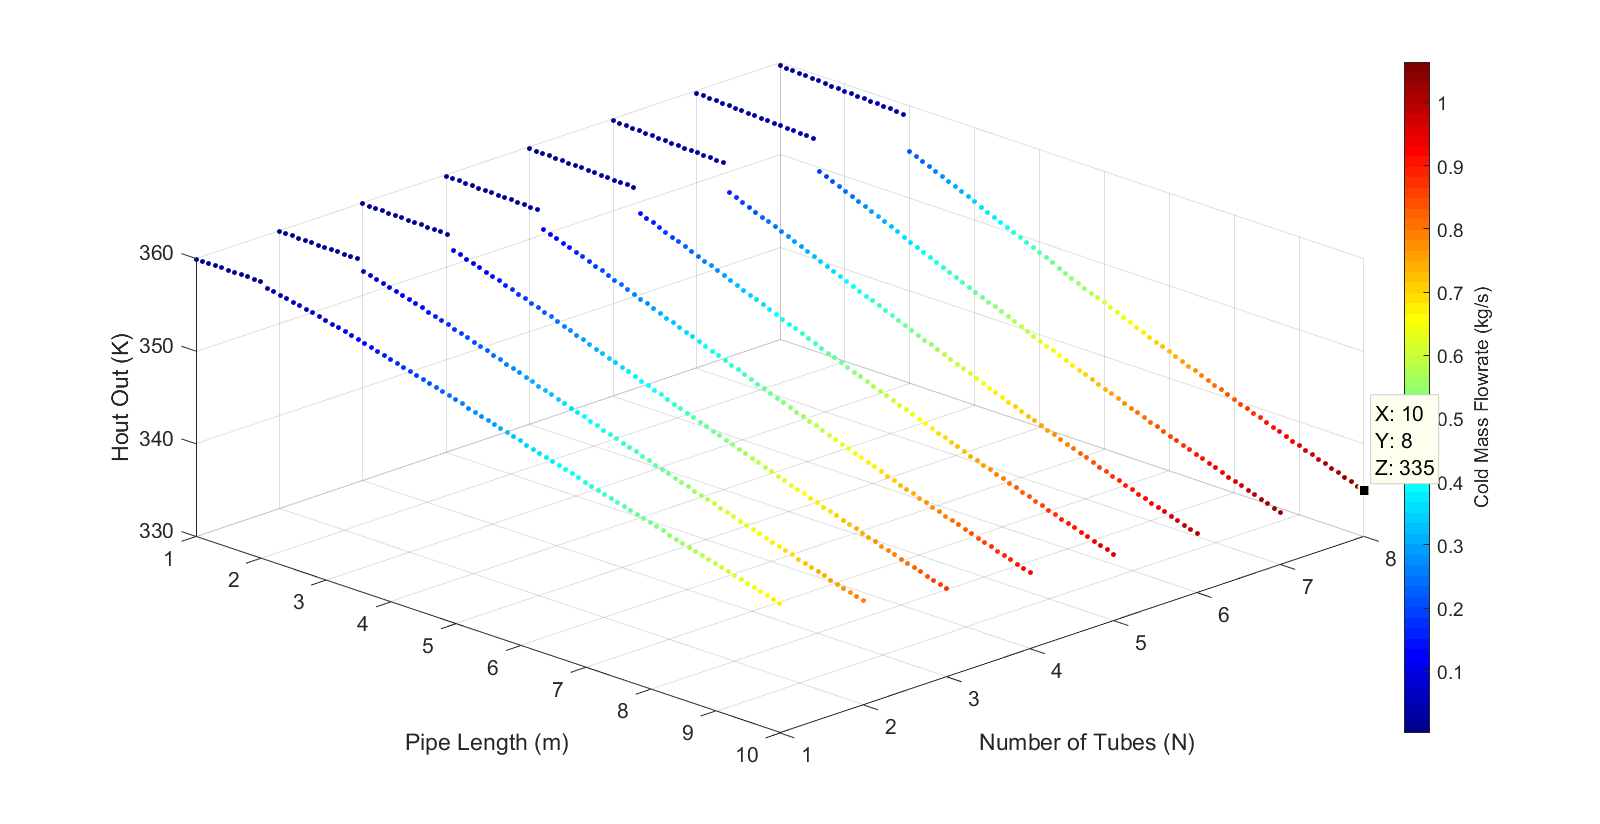
\includegraphics[height=3.5in]{pictures/part_5_mass_a.png}}
\end{figure}
\begin{figure}[H]
  \centering
  \subfloat[Option B - Mass Flowrates]{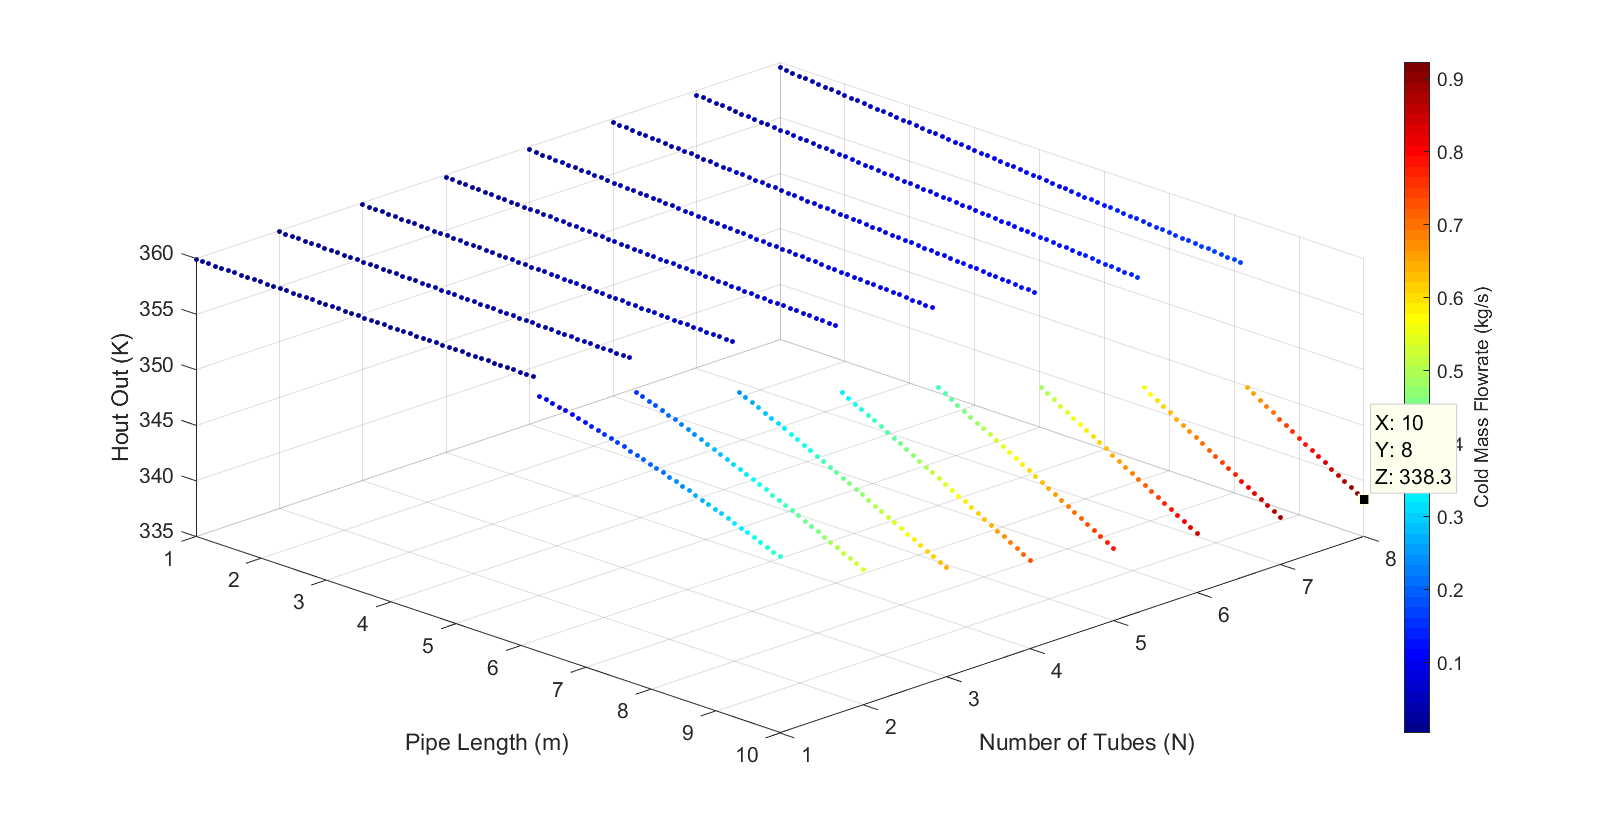
\includegraphics[height=3.5in]{pictures/part_5_mass_b.png}}
\end{figure}
%
\begin{figure}[H]
  \centering
  \subfloat[Option A - Total Effectiveness]{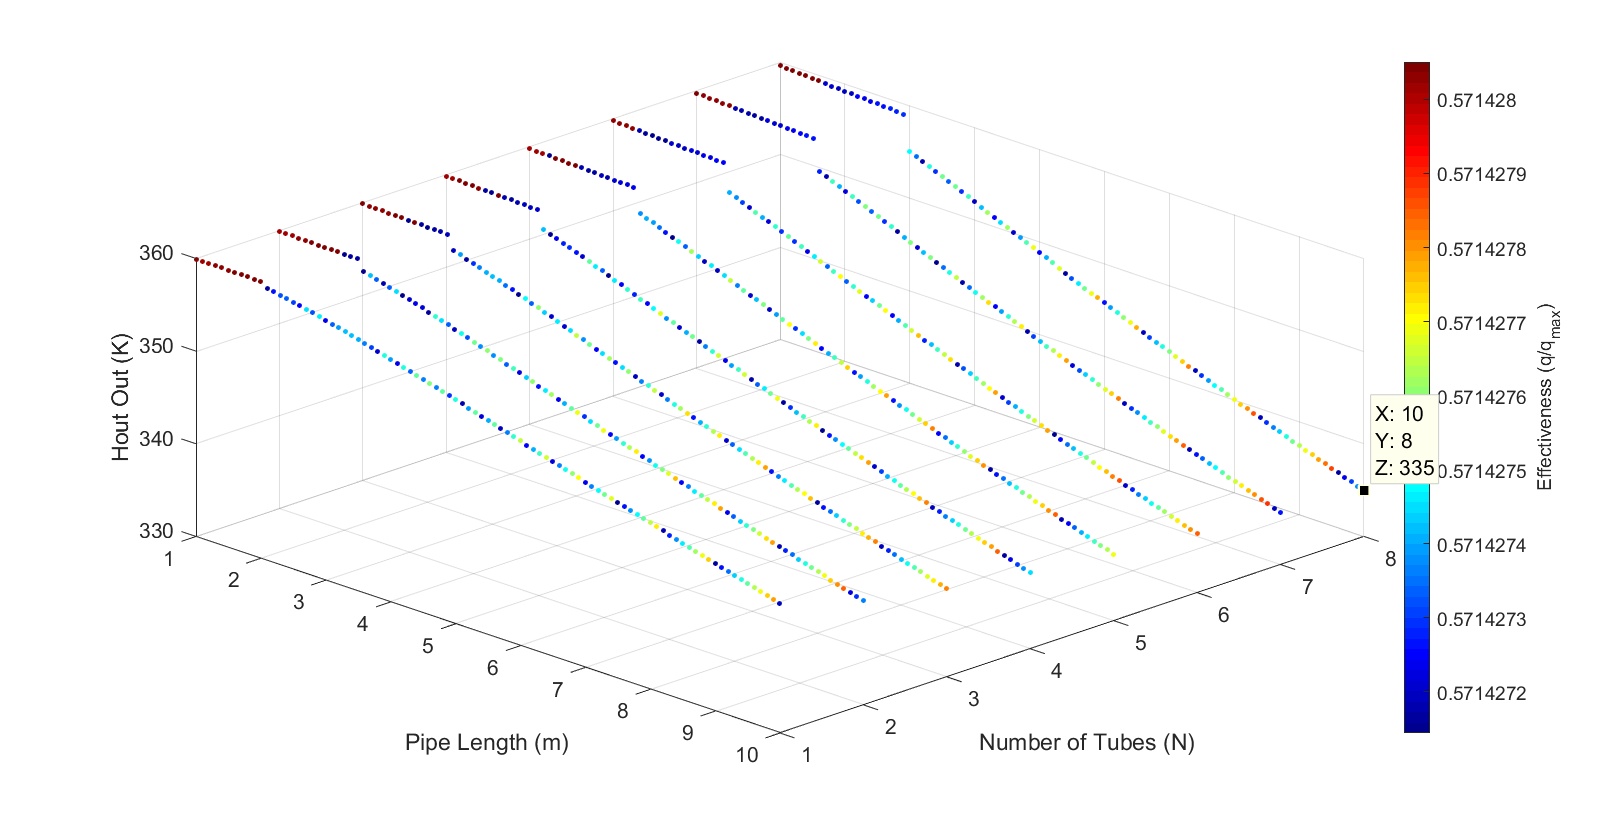
\includegraphics[height=3.5in]{pictures/part_5_eff_a.png}}
\end{figure}
\begin{figure}[H]
  \centering
  \subfloat[Option B - Total Effectiveness]{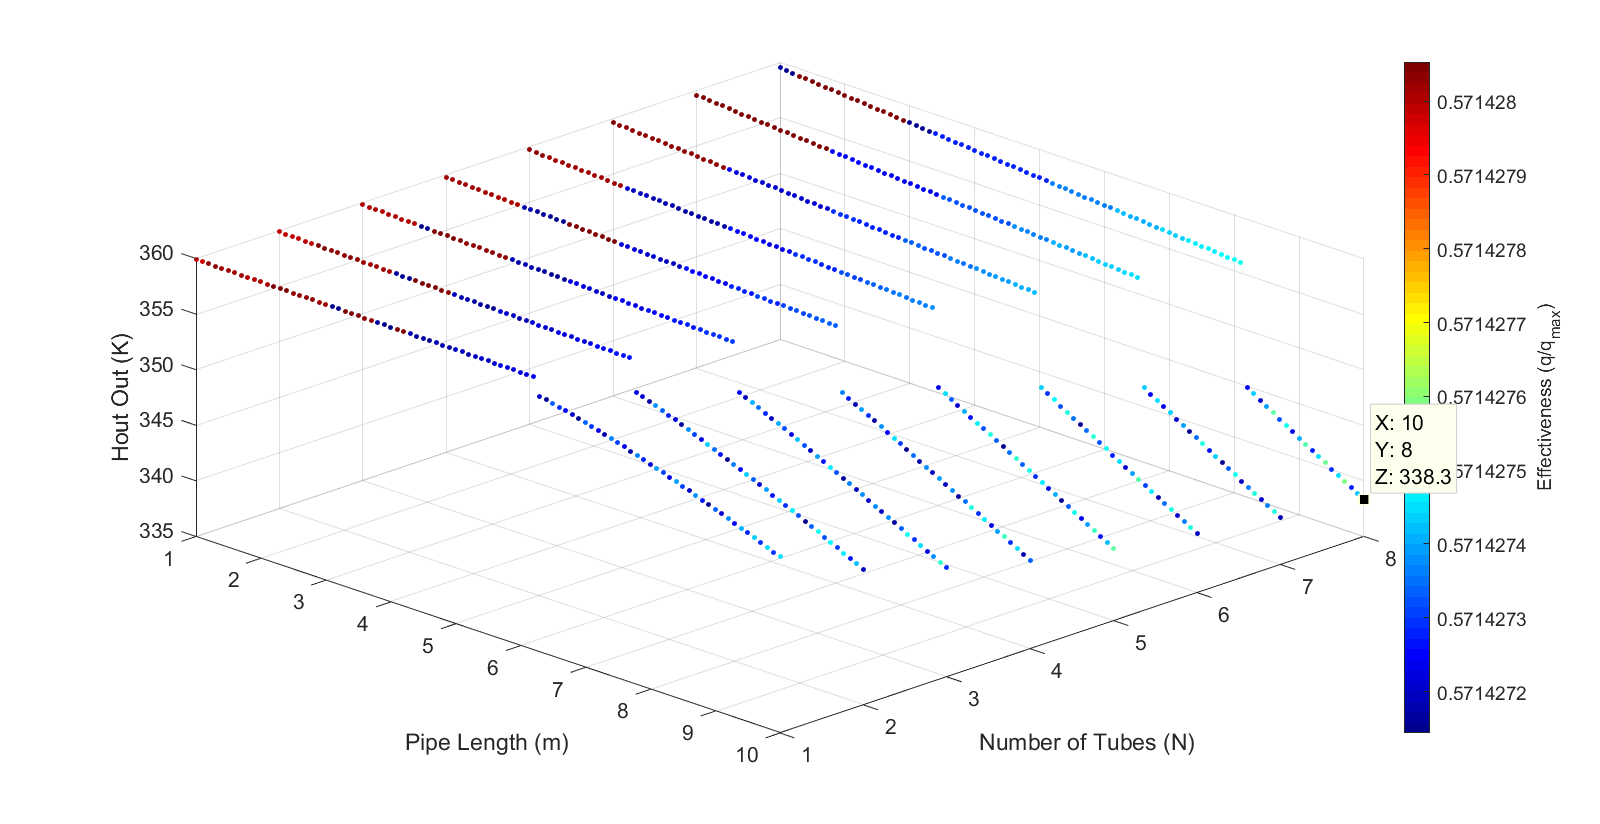
\includegraphics[height=3.5in]{pictures/part_5_eff_b.png}}
\end{figure}
%
\noindent
Also, the previous results showed that Option B would be the better configuration yielding a greater effectiveness, but that figure was produced with a mass flow ratio of 2:1. When the mass flow ratio became less than 1 however, the effectiveness in Option A is actually better than the effectiveness in Option B. Below is a figure that plots how the effectiveness changes with the cold mass flowrate. With a maximum flowrate of 1.064 for Option A and 0.923 for Option B it can be see at these values Option A has a higher efficiency.
%
%  Option A - l = 10  n = 8  Tho = 334.967  eff = 0.57143  m2 = 1.06390
%  Option B - l = 10  n = 8  Tho = 338.294  eff = 0.57143  m2 = 0.92252
%
%
%
\begin{figure}[H]
    \centering
    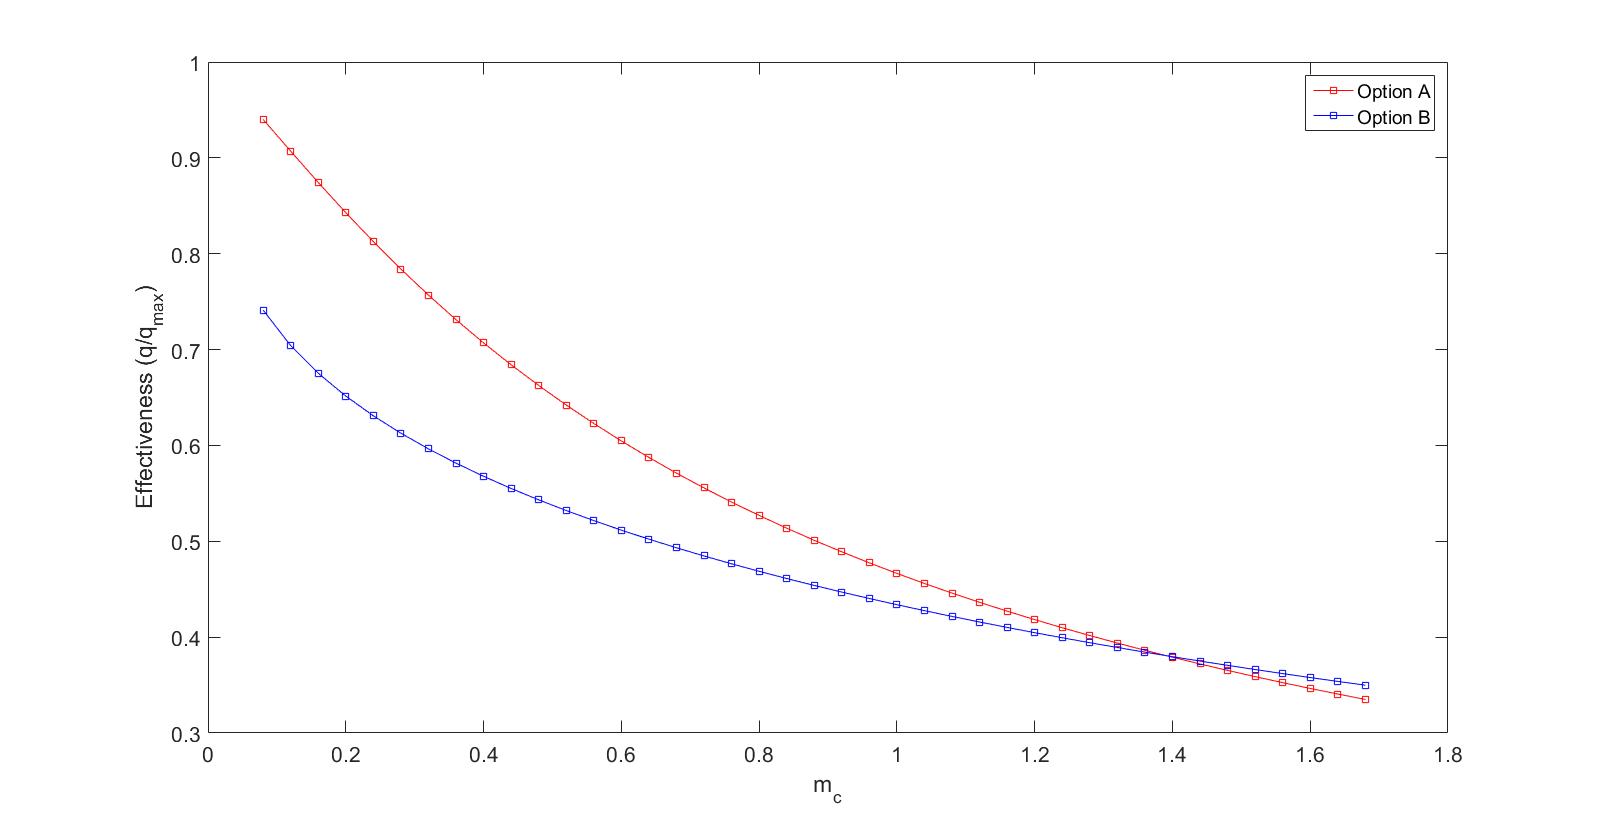
\includegraphics[height=3.5in]{pictures/part_5_eff_cross.png}
\end{figure}
%
\noindent
\textbf{In summary, the design team recommends the construction of a heat exchanger with 8 pipes and with a length of 10. The team recommends that it is configured as Option A with waste water traveling on the outer tube and the cold water traveling in the inner tube. This is backed by the 4D plot comparing the pipe length, number of tubes, Hout, and the cold mass flowrate.}


